\documentclass[letterpaper,12pt,leqno]{article}
\usepackage{paper}
\usepackage{pdflscape}
\bibliographystyle{bibliography}

% Enter paper title:
\hypersetup{pdftitle={Improving Rural Accessibility in Indonesia: Fuel Subsidy versus Infrastructure Development}}

% Enter permanent URL to paper
\codeavailable{https://github.com/maghfiraer/ECON7023-Metrics-II/tree/main/Final_Project}

% Enter BibTeX file with references:
\newcommand{\bib}{bibliography.bib}

% Enter PDF file with figures here:
\newcommand{\pdf}{figures.pdf}

% Fill out paper:
\begin{document}
\title{Improving Rural Accessibility in Indonesia: Fuel Subsidy versus Infrastructure Development}
\author{Maghfira Ramadhani
\thanks{Maghfira Ramadhani: Ph.D. student at Georgia Institute of Technology, maghfira.ramadhani@gatech.edu}}
\date{April 2023}                       
\begin{titlepage}\maketitle

Indonesia has been subsidizing transportation costs for a long time.

\end{titlepage}\section{Introduction}\label{s:introduction}
 
\paragraph{Research question} Although Indonesia has been subsidizing fuel for a long time, high fuel prices were still observed in rural areas in the last decade since they were unable to get the fuel from the official fuel supply chain \citep{liputan_2016, jawapos_2017}. Therefore since 2016, the government initiated the One Price Fuel program to guarantee the availability of subsidized fuel in these areas. The government in collaboration with the National Oil Company started to build a new gas station in the targeted outermost and less-developed village so that they get the fuel at the same price as any other gas station. This program is expected to bring development to the village level by reducing energy costs which could improve the overall village's economic activity. On the other hand, decentralization of development to the village level has been implemented since 2014, when the central government initiate an annual fiscal transfer to the village government to improve their financial capability in bringing development to the last miles\footnote{See Village Law No. 6 of 2014}. This research measures the impact of these government programs in improving rural accessibility at the village level and exercising the efficiency of each specific program.

\paragraph{Answer to the question} In addressing the research question, this research uses unit transportation cost to measure accessibility. Specifically in rural areas, \citet{sambodo_2019} find that transportation spending dominates energy spending which could limit people's mobility and slow economic development. On the other hand, the lack of adequate and reliable infrastructure drives up the transportation cost \citep{sandee_2016}. I treat the unit transportation cost as the willingness to pay for transportation in rural areas, therefore we control for other factors affecting the demand structure to get the causal effect. I use panel data analysis to measure the impact of the two programs in improving rural accessibility. Regarding the fuel program, I obtain the list of 55 government-appointed new distributor locations from the National Oil Company (NOC). I use the village fund transferred to the village government as a proxy for village infrastructure development. From a political economy perspective, infrastructure development is managed by the government directly, while the fuel subsidy is managed through the National Oil Company (NOC) as a delivery agent \citep{ichsan_2022}. This research evaluates the efficiency of the program by comparing the reduction of transportation cost per budget spent as the benefit-cost ratio.

\paragraph{Related literature} This paper builds on the literature on rural development and fossil fuel subsidy in Indonesia. Related literature has indicated that both subsidizing fuel and inter-government transfer contributed to improving the general economic condition in rural areas \citep{sambodo_2019,ichsan_2021,hartojo_2022}. \citep{sambodo_2019} find that villages with better access to energy tend to divert away their spending more productively thus having better health outcomes. \citep{ichsan_2021} argued that the fuel program is a short-term remedy for reducing transportation costs in rural areas, and believes that infrastructure development is the sustainable way to do so. On the effect of village fund transfer, \citet{hartojo_2022} show that the transfer effectively improved rural economic growth in rural areas. This research is the first to evaluate and compare the impact of both programs in improving accessibility at the village level.

\paragraph{Outline} The rest of the paper is organized as follows. I develop the institutional context and conceptual framework for the discussion in Section \ref{s:framework}. Section \ref{s:data} describes the data and its summary statistics. Section \ref{s:result} discusses the findings and provides a robustness check and evaluates the benefit-cost of the programs. Section \ref{s:conclusion} provides a concluding remark of the discussion.

\section{Institutional Context and Conceptual framework}\label{s:framework}

In this section, I discussed the institutional context of Indonesia and build a conceptual framework for understanding the impact of how the fossil fuel program and village development can improve rural accessibility.

\subsection{Accessibility in rural area}

\paragraph{Accessibility challenge in Indonesia}
Following \citet{sandee_2016}, regarding rural accessibility in Indonesia, the challenge mainly related to intra-island connectivity ---links within individual islands--- is linking underdeveloped regions to growth centers. In the densely populated part of Java island, the city is the center of growth, the challenges of connectivity are mostly congestion-based challenges causing high-cost for mobility. In contrast, in the rural areas of Java, we can still find a village that we can only access by motorcycle or even only by foot. This challenge is somewhat similar in other main islands such as Sumatra, Kalimantan, Sulawesi, and Papua. In these other mainlands, the challenges are the existence of adequate and reliable infrastructure that drives up transportation costs. The government initiatives in attracting foreign capital and facilitating public-private partnerships in bringing a large-scale infrastructure development have been a policy priority since 2015 \citep{pwc_2016}.


\paragraph{Transportation cost as a measure of accessibility} We can treat unit transportation cost as the willingness to pay or demand for transportation. We follow previous literature on willingness to pay for rural transportation from revealed preference, the affecting factors include travel time, convenience, and trip purpose i.e. work or education.



\subsection{Fossil fuel subsidy regime}

Indonesia used to be a large oil exporter in the oil boom period in the 1970s and 1980s and the National Oil Company (NOC), Pertamina contributed a big part in delivering the fuel subsidy to the public \citep{ichsan_2022}. However, as the production declined, there has been increased pressure for subsidy reform. 

\subsection{Decentralization of development}

Developing countries believe decentralization and local government reform are more efficient in bringing local development \citep{vazquez_2017} and providing public goods better than central government \citep{arends2020}. In 2014 the government enacted village fund transfer to implement decentralization at the village level. The allocation amount takes into account village conditions, i.e. poverty and geographic difficulty into account.

\section{Data}\label{s:data}

I obtained the Village Potential Statistics data for the years 2014 and 2018 from Indonesia's Central Bureau of Statistics complemented with village fund transfer data from the Ministry of Village Development.

I measure rural accessibility using the unit transportation cost (in Rp/km) of each individual village $i$ for year $t$. I define unit transportation cost, $y_{it}$, as the transportation cost from the village $i$'s office to the sub-district office (in thousands Rp) at year $t$, $c_{it}$, divided by the distance from the village office $i$'s to the sub-district office (in km) at year $t$, $d_{it}$.
\begin{equation}
        y_{it}=d_{it}/c_{it}    
\end{equation}

I obtain the list of 55 government-appointed new distributor's village locations from the NOC and then define all the villages that are in the same sub-district as treated by the program, i.e. $D_{it}=1$ in the year 2018. Note in the year 2014 all $D_{it}=0$. 

For example, suppose the government in 2016 gives the order for the NOC to build a new distribution point at village $A$. Village $A$ is in the same sub-district as villages $B,C$, and $D$. Then all villages $A,B,C$, and $D$ are treated.

Other data on geographic characteristics, i.e land topography, region boundary with forest or sea, river transportation use, and poverty can be used as covariates or instruments.


\section{Empirical strategy}\label{s:strategy}

I observed village level as the unit of analysis. I obtained a proprietary Village Potential Statistics data for the year 2011, 2014 and 2018 from Indonesia's Central Bureau of Statistics consisting of consecutively 77,961, 82,190, and 83,931 observations of village in rural and urban areas. The original survey covers the general information of village, population and employment, housing and environment, natural disaster, education and health, sport and leisure, transportation and communication, land use, economic activity, security, local government, community empowerment, and agriculture. However, the data on transportation cost are not collected in the year 2011, and also the data about village government budget is not available for the year 2018.  

\subsection{Measuring rural accessibility with transportation cost}



\section{Results}\label{s:result}
\subsection{Preliminary findings}



\paragraph{Another paragraph} At vero eos et accusamus et iusto odio dignissimos ducimus, qui blanditiis praesentium voluptatum deleniti atque corrupti, quos dolores et quas molestias excepturi sint, obcaecati cupiditate non provident, similique sunt in culpa, qui officia deserunt mollitia animi, id est laborum et dolorum fuga. Et harum quidem rerum facilis est et expedita distinctio. Nam libero tempore, cum soluta nobis est eligendi optio, cumque nihil impedit, quo minus id, quod maxime placeat, facere possimus, omnis voluptas assumenda est, omnis dolor repellendus. Temporibus autem quibusdam et aut officiis debitis aut rerum necessitatibus saepe eveniet, ut et voluptates repudiandae sint et molestiae non recusandae. Itaque earum rerum hic tenetur a sapiente delectus, ut aut reiciendis voluptatibus maiores alias consequatur aut perferendis doloribus asperiores repellat. 

\paragraph{Yet another paragraph} At vero eos et accusamus et iusto odio dignissimos ducimus, qui blanditiis praesentium voluptatum deleniti atque corrupti, quos dolores et quas molestias excepturi sint, obcaecati cupiditate non provident, similique sunt in culpa, qui officia deserunt mollitia animi, id est laborum et dolorum fuga. Et harum quidem rerum facilis est et expedita distinctio. Nam libero tempore, cum soluta nobis est eligendi optio, cumque nihil impedit, quo minus id, quod maxime placeat, facere possimus, omnis voluptas assumenda est, omnis dolor repellendus. Temporibus autem quibusdam et aut officiis debitis aut rerum necessitatibus saepe eveniet, ut et voluptates repudiandae sint et molestiae non recusandae. Itaque earum rerum hic tenetur a sapiente delectus, ut aut reiciendis voluptatibus maiores alias consequatur aut perferendis doloribus asperiores repellat. 



\section{Conclusion}\label{s:conclusion}

To conclude, at vero eos et accusamus et iusto odio dignissimos ducimus, qui blanditiis praesentium voluptatum deleniti atque corrupti, quos dolores et quas molestias excepturi sint, obcaecati cupiditate non provident, similique sunt in culpa, qui officia deserunt mollitia animi, id est laborum et dolorum fuga. 

At vero eos et accusamus et iusto odio dignissimos ducimus, qui blanditiis praesentium voluptatum deleniti atque corrupti, quos dolores et quas molestias excepturi sint.

\bibliography{\bib}

% Fill out appendix:
\newpage
\appendix
\begin{landscape}
\section{Tables}\label{a:table}

\begin{table}[h]
\caption{Summary statistics of main variables with the province-level as sample} 
\scalebox{0.85}{\begin{tabular}{l*{2}{ccccc}}
\toprule
                &     2014&         &         &         &         &     2018&         &         &         &         \\
                &     Mean&     S.D.&      Min&      Max&     Obs.&     Mean&     S.D.&      Min&      Max&     Obs.\\
\midrule
\emph{Transportation}&         &         &         &         &         &         &         &         &         &         \\
\hspace{0.25cm} Unit transportation cost in 000s Rp./km&     3.29&    19.94&     0.00&  1000.00&    38624&     3.22&     9.36&     0.00&   800.00&    38646\\
\hspace{0.25cm} Travel duration (hrs)&     1.17&     1.44&     1.00&    99.00&    38624&     0.50&     1.41&     0.00&    60.50&    38646\\
\vspace{0.05em} \\ \emph{Natural Disaster}&         &         &         &         &         &         &         &         &         &         \\
\hspace{0.25cm} Landfall occurence average per year&     0.11&     0.52&     0.00&     9.00&    38624&     0.15&     0.62&     0.00&     9.00&    38646\\
\hspace{0.25cm} Earthquake occurence average per year&     0.04&     0.29&     0.00&     9.00&    38624&     0.23&     1.07&     0.00&     9.00&    38646\\
\vspace{0.05em} \\ \emph{Infrastructure}&         &         &         &         &         &         &         &         &         &         \\
\hspace{0.25cm} Number of PLN electricity user household&   656.51&   781.91&     0.00& 14460.00&    38624&   738.27&   887.98&     0.00& 17530.00&    38646\\
\hspace{0.25cm} Number of Junior High School&     0.53&     0.82&     0.00&    14.00&    38624&     0.58&     0.86&     0.00&    12.00&    38646\\
\hspace{0.25cm} Number of Senior High School&     0.26&     0.70&     0.00&    40.00&    38624&     0.31&     0.74&     0.00&    11.00&    38646\\
\vspace{0.05em} \\ \emph{Inter-government Transfer}&         &         &         &         &         &         &         &         &         &         \\
\hspace{0.25cm} Revenue from village fund transfer&   116.08&   213.26&     0.00&  7716.00&    38624&   121.07&   143.42&     0.00& 13662.00&    36630\\
\bottomrule
\end{tabular}
}
\note{Temporibus autem quibusdam et aut officiis debitis aut rerum necessitatibus saepe eveniet, ut et voluptates repudiandae sint et molestiae non recusandae. Ut aut reiciendis voluptatibus maiores alias consequatur aut perferendis doloribus asperiores repellat}
\label{t:1}\end{table}


\begin{table}[h]
\caption{Summary statistics of main variables with the district-level as sample} 
\scalebox{0.85}{\begin{tabular}{l*{2}{ccccc}}
\toprule
                &     2014&         &         &         &         &     2018&         &         &         &         \\
                &     Mean&     S.D.&      Min&      Max&     Obs.&     Mean&     S.D.&      Min&      Max&     Obs.\\
\midrule
\emph{Transportation Cost}&         &         &         &         &         &         &         &         &         &         \\
\hspace{0.25cm} Unit transportation cost in 000s Rp./km&     5.14&    21.02&     0.00&  1000.00&     3407&     4.93&    12.47&     0.00&   400.00&     3411\\
\hspace{0.25cm} Travel Duration&     1.27&     1.27&     1.00&    30.00&     3407&     0.74&     2.36&     0.00&    60.50&     3411\\
\vspace{0.05em} \\ \emph{Natural Disaster}&         &         &         &         &         &         &         &         &         &         \\
\hspace{0.25cm} Landfall occurence average per year&     0.07&     0.37&     0.00&     6.00&     3407&     0.10&     0.49&     0.00&     9.00&     3411\\
\hspace{0.25cm} Earthquake occurence average per year&     0.04&     0.35&     0.00&     7.00&     3407&     0.46&     1.60&     0.00&     9.00&     3411\\
\vspace{0.05em} \\ \emph{Infrastructure}&         &         &         &         &         &         &         &         &         &         \\
\hspace{0.25cm} Number of PLN electricity user household&   366.92&   610.20&     0.00&  6726.00&     3407&   422.79&   651.77&     0.00&  6468.00&     3411\\
\hspace{0.25cm} Number of Junior High School&     0.54&     0.85&     0.00&     9.00&     3407&     0.61&     0.89&     0.00&    12.00&     3411\\
\hspace{0.25cm} Number of Senior High School&     0.27&     0.66&     0.00&     7.00&     3407&     0.33&     0.73&     0.00&     8.00&     3411\\
\vspace{0.05em} \\ \emph{Inter-government Transfer}&         &         &         &         &         &         &         &         &         &         \\
\hspace{0.25cm} Revenue from village fund transfer&   113.55&   129.92&     0.00&  1253.00&     3407&   158.93&   289.35&     0.00& 13662.00&     3172\\
\bottomrule
\end{tabular}
}
\note{Temporibus autem quibusdam et aut officiis debitis aut rerum necessitatibus saepe eveniet, ut et voluptates repudiandae sint et molestiae non recusandae. Ut aut reiciendis voluptatibus maiores alias consequatur aut perferendis doloribus asperiores repellat}
\label{t:2}\end{table}
\end{landscape}

\section{Figures}

\begin{figure}[h]
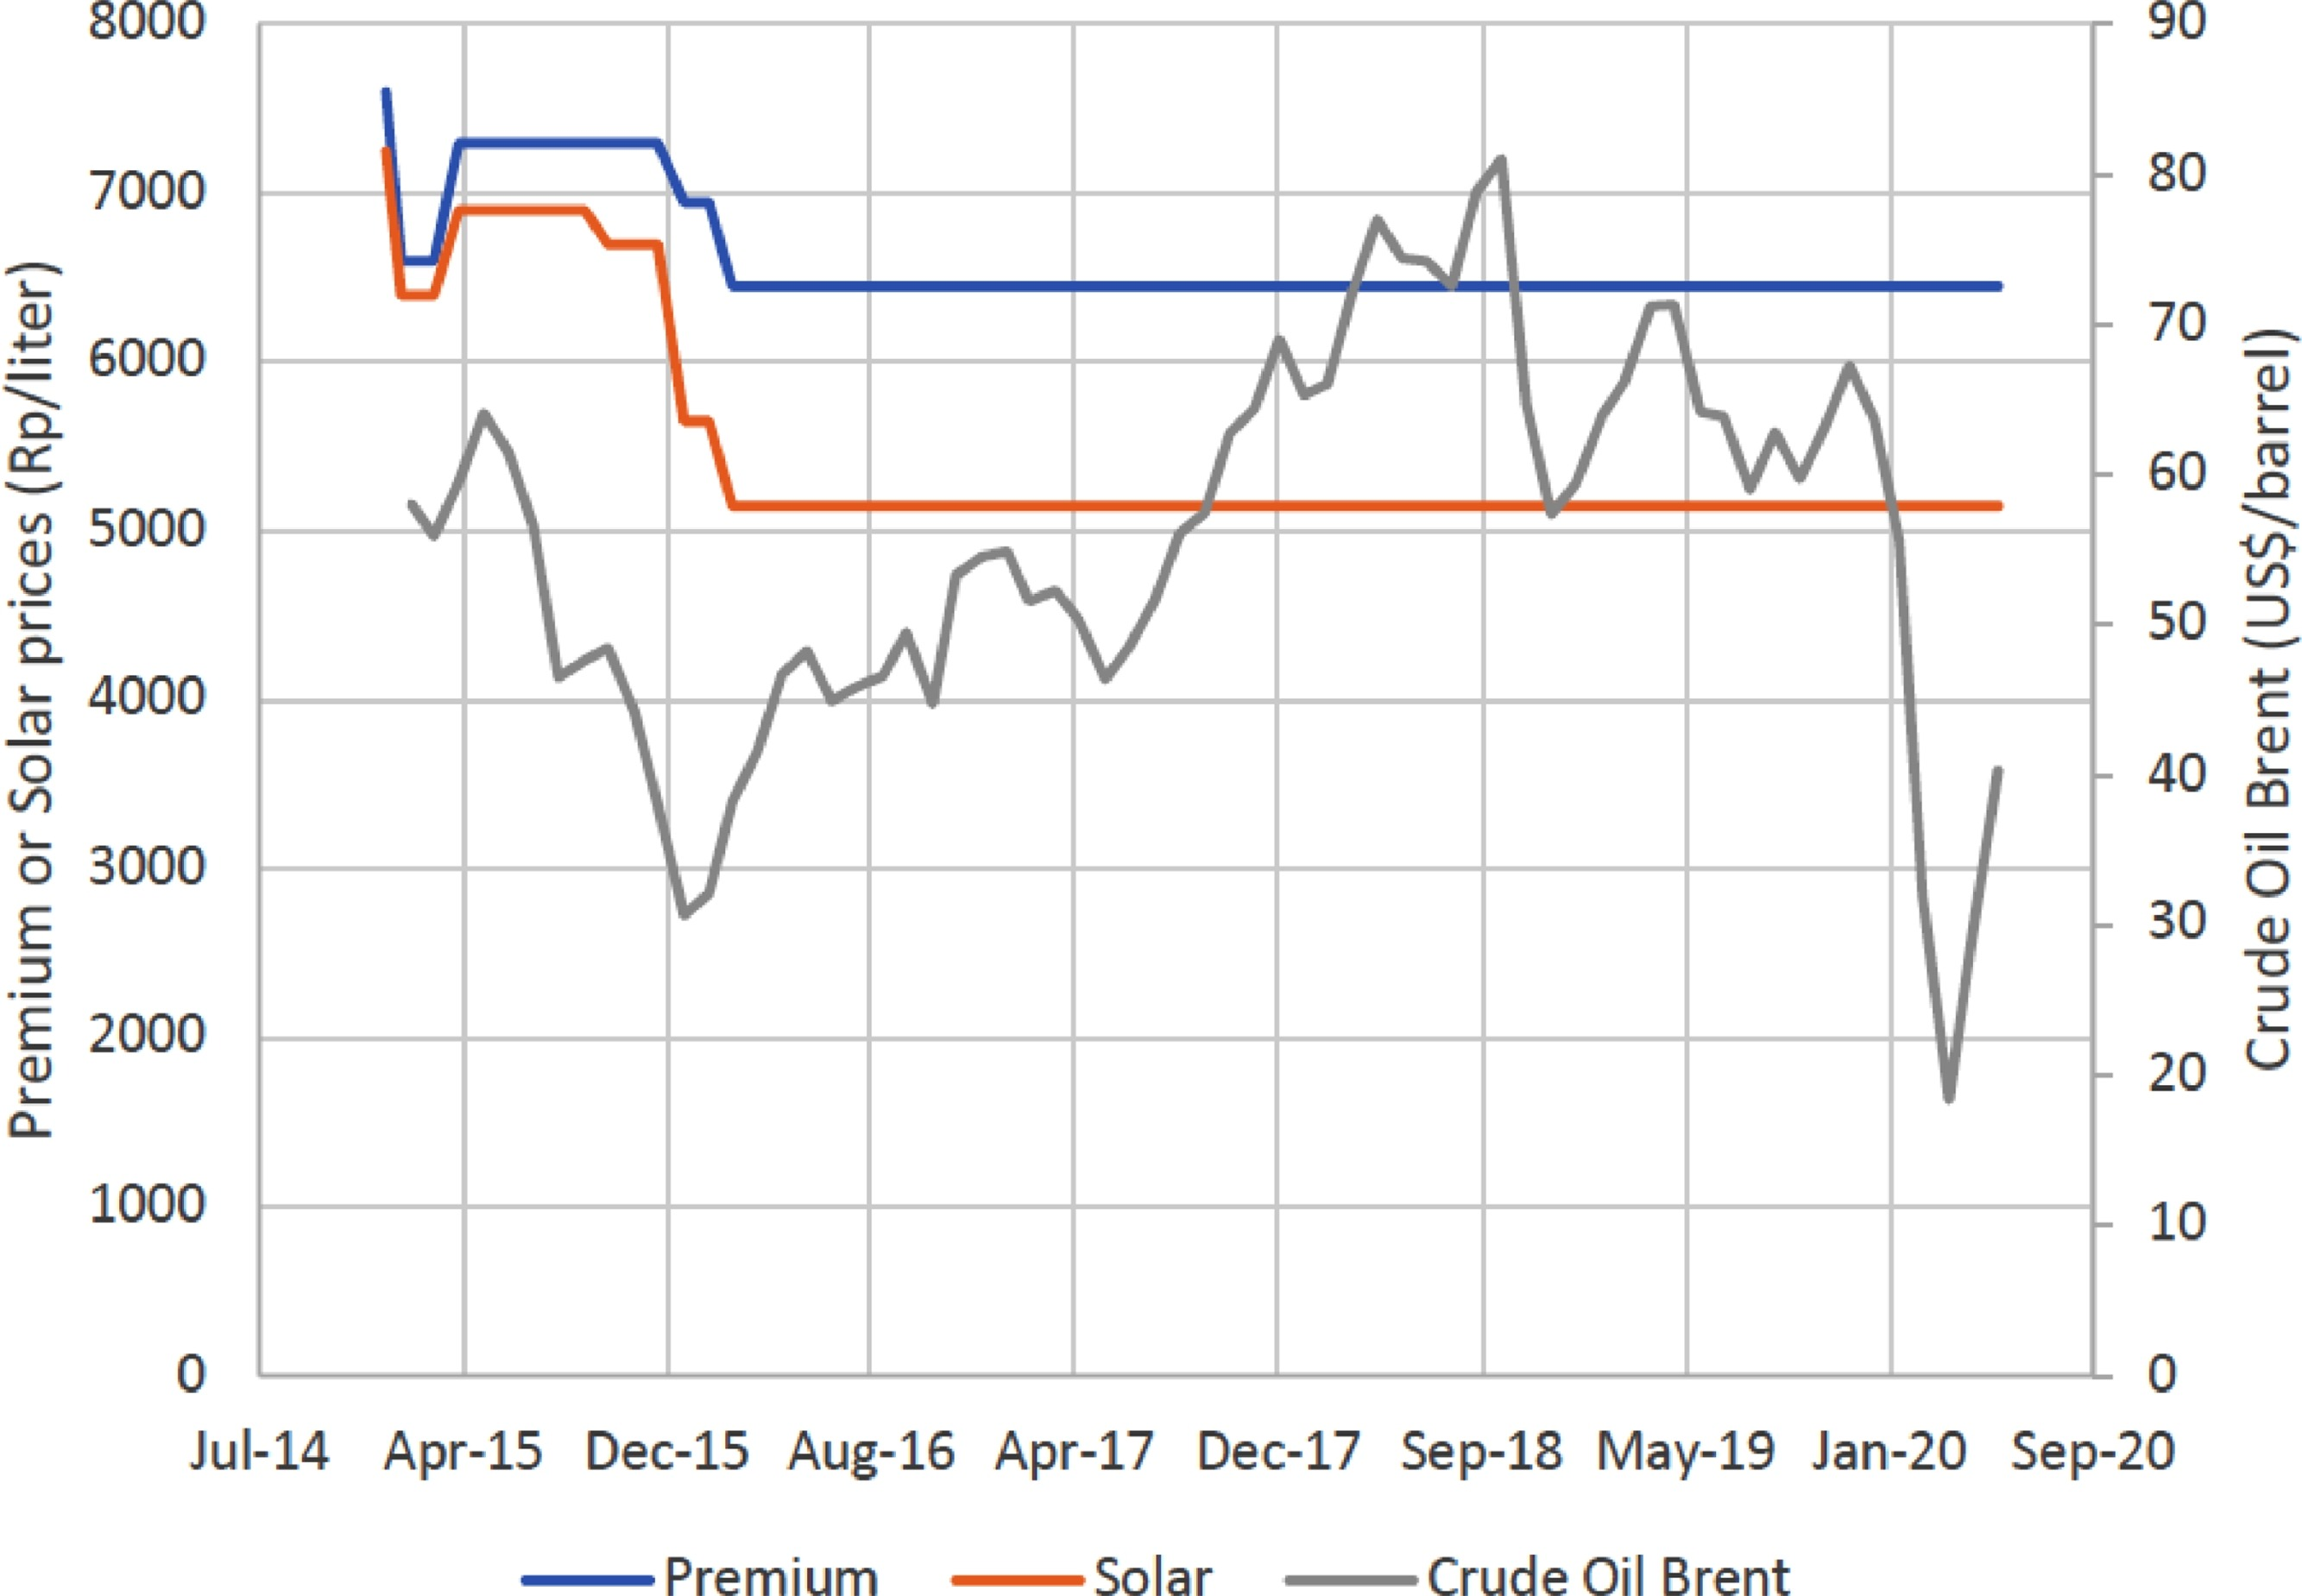
\includegraphics[scale=0.7]{Final_Project/image/bbm-price-2014-2018.jpg}
\caption{Subsidized Fuel Price at Government's Price Control 2014-2018}
\note{Source: \citet{ichsan_2022}}
\label{f:graph1}
\end{figure}

\begin{figure}[h]
\subcaptionbox{Village status in 2014\label{f:panel1}}{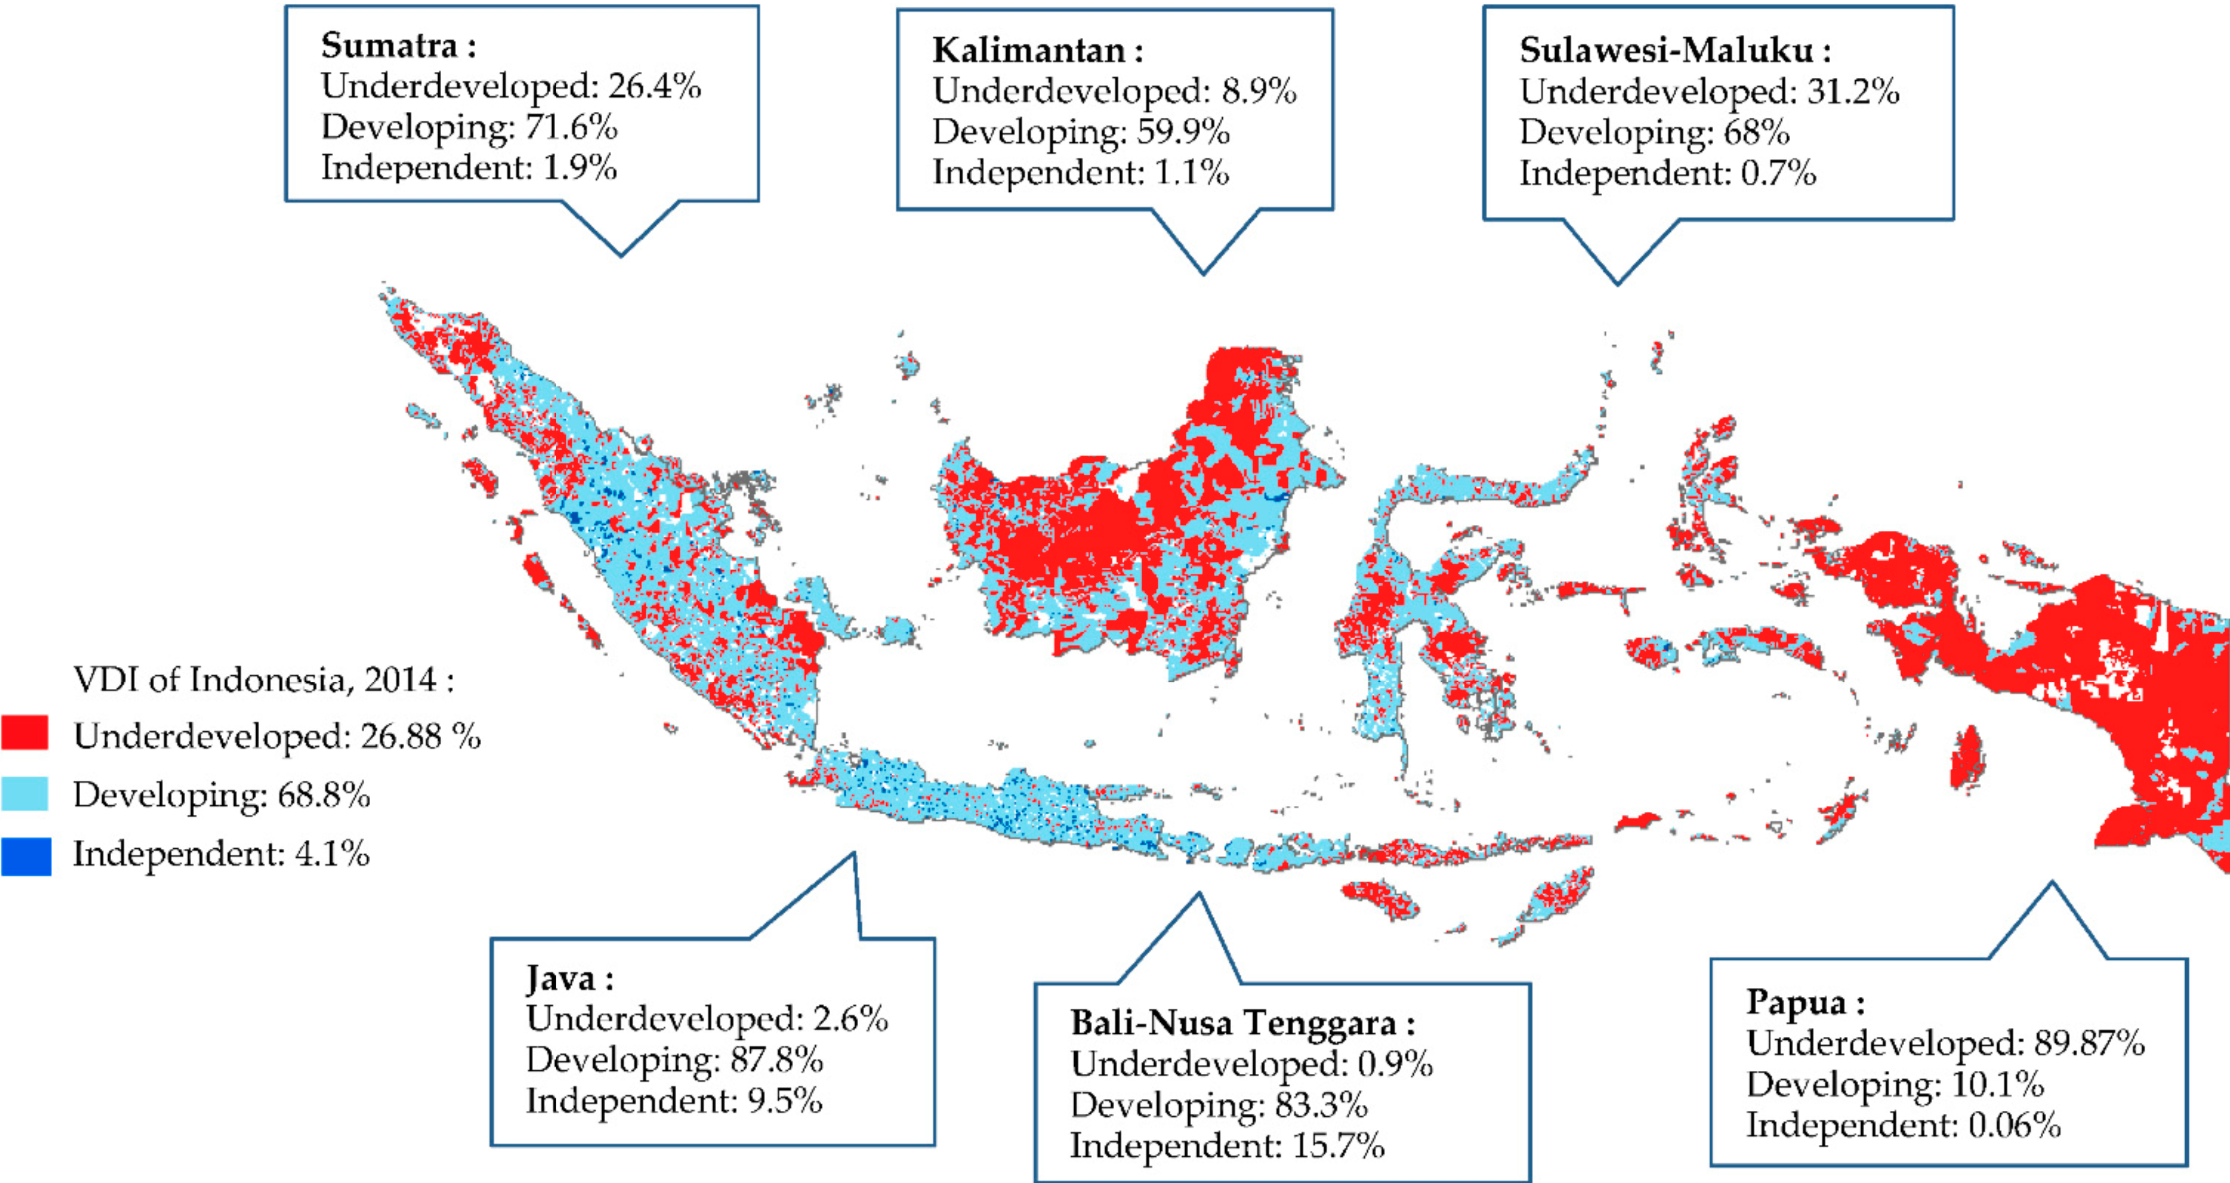
\includegraphics[scale=0.2]{Final_Project/image/vdi2014.png}}\hfill
\subcaptionbox{Village status in 2018\label{f:panel2}}{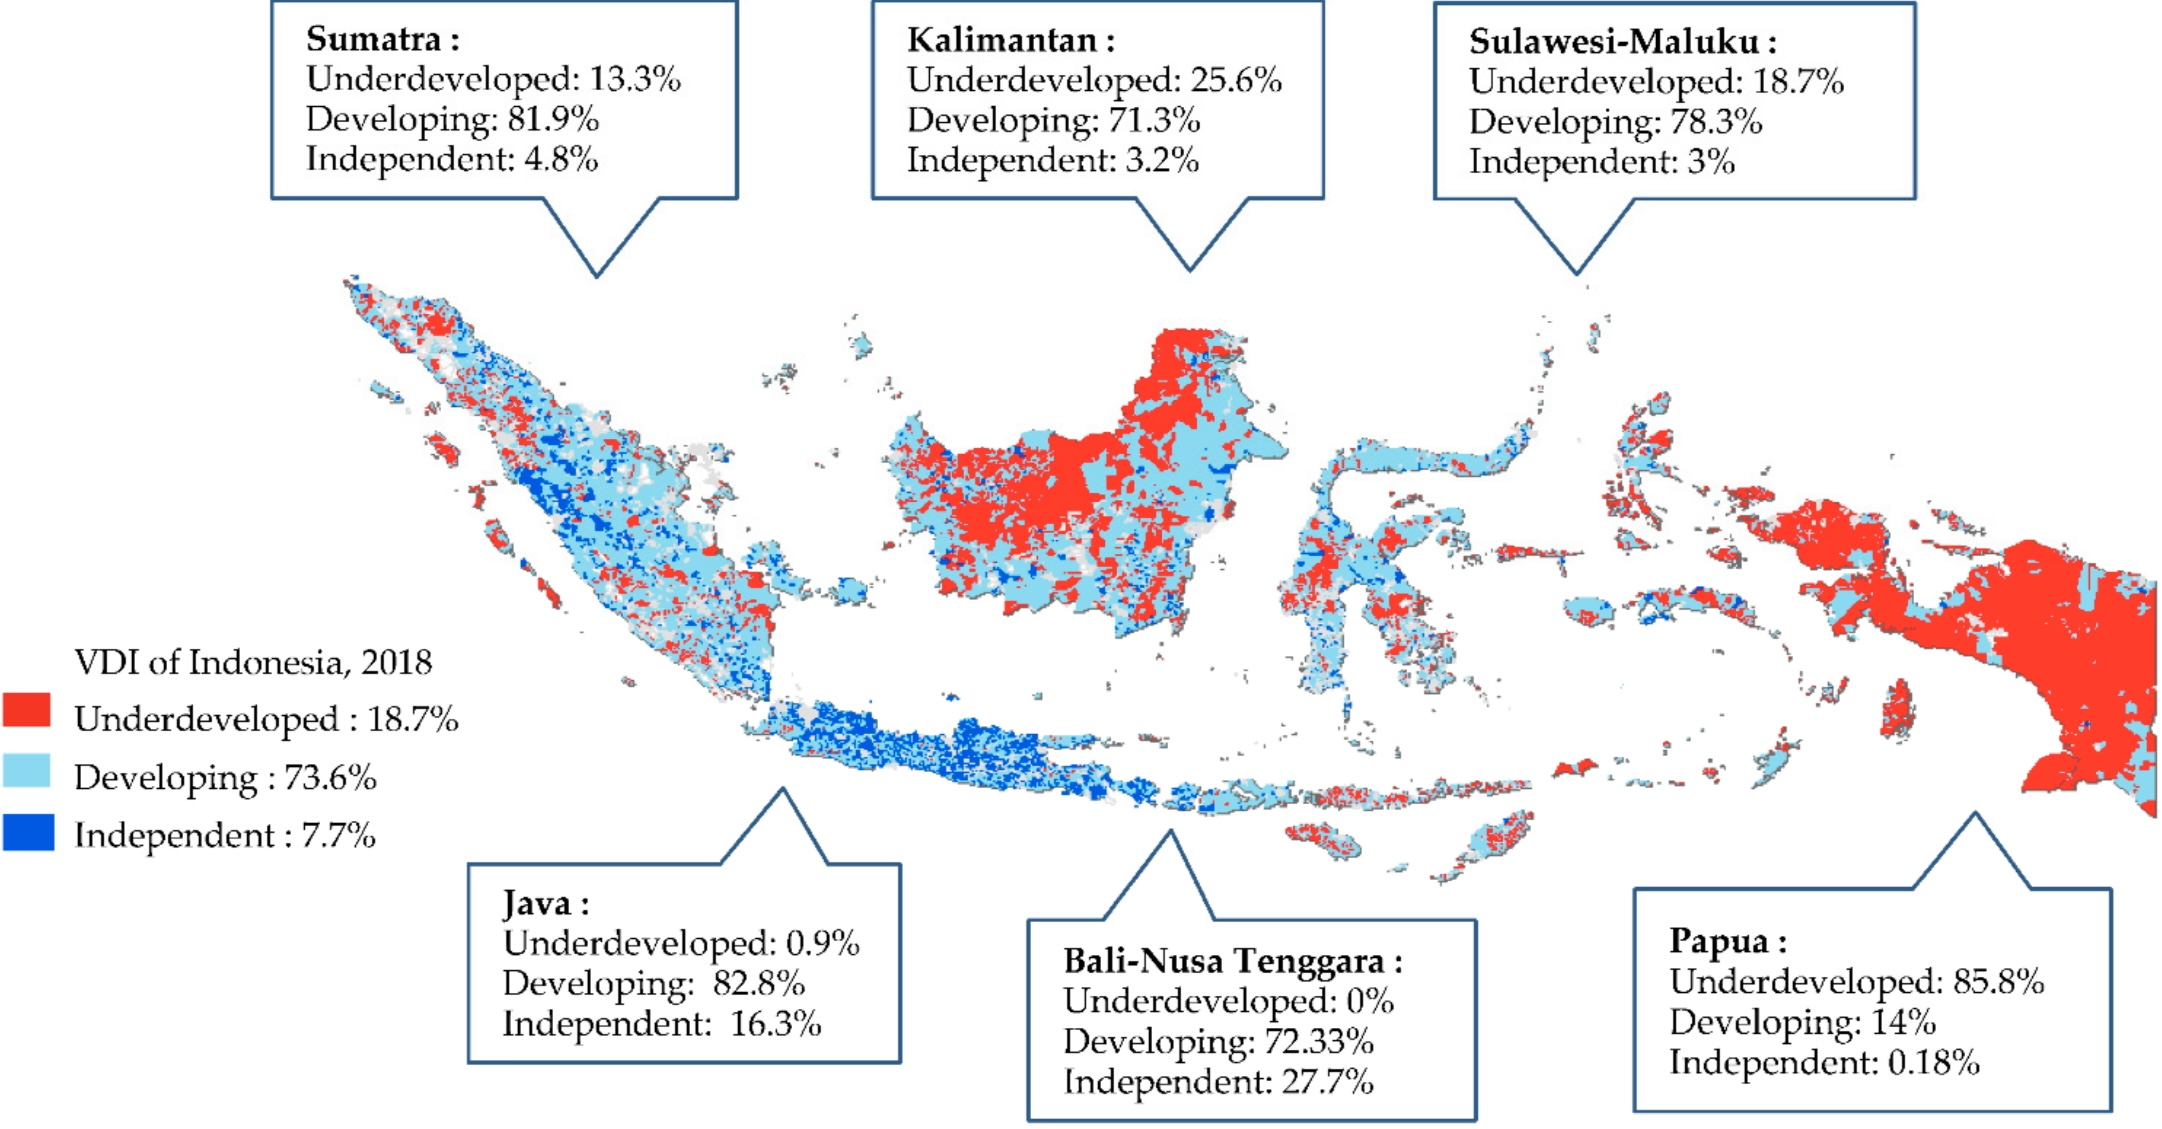
\includegraphics[scale=0.205]{Final_Project/image/vdi2018.jpg}}
\caption{Indonesia's Village Development Index status}
\note{Source: Statistics Indonesia from \citet{hartojo_2022}}
\label{f:1}\end{figure}
 


\section{Another section}\label{a:appendix2}

At vero eos et accusamus et iusto odio dignissimos ducimus, qui blanditiis praesentium voluptatum deleniti atque corrupti.

\subsection{Even larger figure, without panel, in the appendix} 

At vero e

\subsection{Final subsection with footnote and references}\label{a:subappendix}

Nemo enim ipsam voluptatem quia voluptas sit aspernatur aut odit aut fugit, sed quia consequuntur magni dolores eos qui ratione voluptatem sequi nesciunt $\mathcal{V}^i > \mathcal{V}^r$ \citep{MS21b}.\footnote{The reference goes to the reference list at the end of the main text.} Sed ut perspiciatis unde omnis iste natus error sit voluptatem accusantium doloremque laudantium, totam rem aperiam, eaque ipsa quae ab illo inventore veritatis et quasi architecto beatae vitae dicta sunt explicabo. This results are summarized in a repository with the following URL: \url{https://github.com/pmichaillat/latex-paper}.


\end{document}
